\chapter{Videospiele}
\label{chap:videospiele}

Das Grundlagenkapitel zu Videospielen definiert den Begriff sowie die verschiedenen Perspektiven und Genres von Videospielen.

Bei Videospielen handelt es sich um interaktive Medien, die Spielern eine immersive und unterhaltsame Erfahrung bieten. Sie erm\"{o}glichen eine Interaktion zwischen einem Spieler, einer Hardware und gelegentlich weiteren Spielern. Diese Interaktion erfolgt mithilfe von Eingabeger\"{a}ten in einer fiktionalen Spielwelt. Bei den Eingabeger\"{a}ten kann es sich um eine Maus, Tastatur, Gamepad oder Touch-Display handeln. Die fiktionale Spielwelt wird \"{u}ber die Ausgabeger\"{a}te der Hardware visuell, akustisch oder haptisch simuliert. Innerhalb des Videospiels wird der Spieler durch seine Handlungen und Konsequenzen emotional beeinflusst. \autocite{Bergonse}

\section{Perspektiven}
\label{chap:perspektiven}

Nicht nur Filme und Literatur, sondern auch Videospiele werden von ihrem Nutzer \"{u}ber eine Perspektive erfasst. So werden Filme \"{u}ber verschiedene Kameraperspektiven gedreht, die auch in Videospielen vorhanden sind. In Videospielen spricht man von den folgenden Perspektiven: Third-Person und First-Person.

Die Third-Person-Perspektive ist eine Perspektive au\ss{}erhalb der gesteuerten Spielfigur und kommt in 2D und 3D Umgebung sowie in allen Genres vor.

Das Gegenst\"{u}ck zu der Third-Person-Perspektive ist die First-Person-Perspektive, die auch als Egoperspektive bezeichnet wird. Bei dieser handelt es sich um eine Perspektive aus den Augen der Spielfigur.

\section{Genres}
\label{chap:genres}

Genres kategorisieren k\"{u}nstlerische Werke nach ihren Eigenschaften, wie nach ihrem Inhalt und ihrer Art. Sowohl Filme, Musik und Literatur als auch Videospiele z\"{a}hlen zu k\"{u}nstlerischen Werken. So lassen sich Videospiele nach ihrem Spielinhalt und ihrer Spielart unterteilen. Klassische Videospiel-Genres sind Renn-, Rollen-, Strategiespiel, Horror und Shooter. Ein Videospiel muss nicht ausschlie\ss{}lich einem Genre angeh\"{o}ren, sondern kann auch mehreren Genres zugeordnet werden. So f\"{a}llt das Videospiel F.E.A.R (2005) in die folgenden beiden Genres: Horror und Shooter.

Videospiel-Genres werden wiederum durch Subgenres nach ihren Darstellungen, Perspektiven und Spielmechaniken unterteilt. So k\"{o}nnen Videospiele des Genre Shooter entweder in der 2D oder 3D Umgebung spielen. Je nach Perspektive wird ein Shooter entweder als Third-Person-Shooter (TPS) oder als First-Person-Shooter (FPS) bezeichnet. Spielmechaniken beeinflussen die Spielweise des Videospielers. Unter anderem gibt es Spielmechaniken, die dem Spieler die M\"{o}glichkeit geben, K\"{a}mpfe durch Schleichen zu vermeiden. Shooter mit dieser Spielmechanik werden als Stealth-Shooter bezeichnet. Im Gegensatz zum Stealth-Shooter zwingt der Action-Shooter den Spieler aktiv zum Kampf, wie im Videospiel F.E.A.R. Die Abbildung \ref{fig:fps tps} stellt einen First-Person-Shooter und Third-Person-Shooter dar.

\begin{figure}[h]
  \centering
  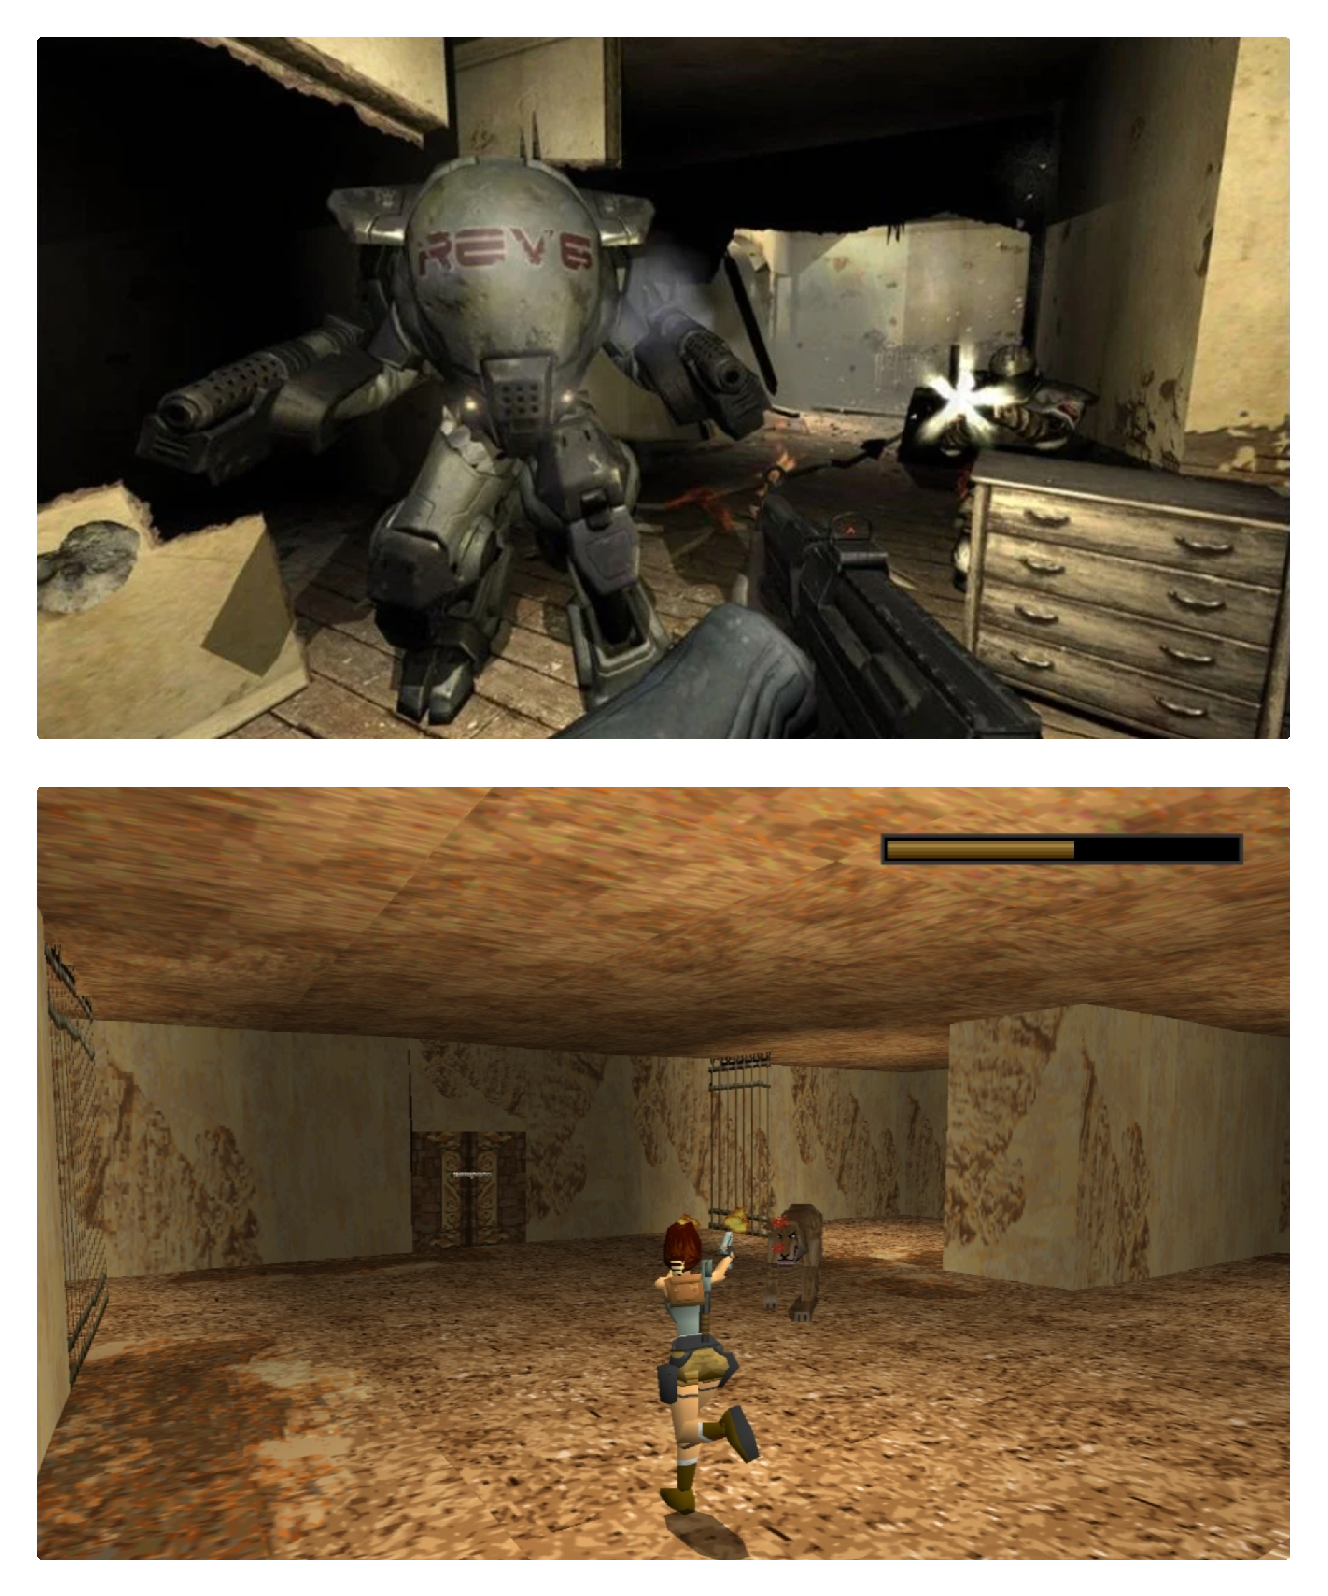
\includegraphics[width=0.75\textwidth]{Videospiele/fps tps}
	\captionsetup{justification=justified, format=plain}
  \caption{First-Person-Shooter: F.E.A.R (2005) (oben) und Third-Person-Shooter: Tomb Raider (1996) (unten)}
  \label{fig:fps tps}
\end{figure}


